\documentclass[10pt, letterpaper]{memoir}
\usepackage{HomeworkStyle}

\begin{document}
\begin{center}
	{\large Homework 12 -- Rotational and Vibrational Spectra}
	
	Due: Friday, March 30 \hspace{3em} Points: ${\dfrac{~}{~~50~~}}$
\end{center}

Name: \rule[-.1mm]{15em}{0.1pt}	
	
	\section*{Problem 1 (10 points)}
	These are infrared spectra for (in no particular order) a $\circ$ Nitrile, $\circ$ Alkane, $\circ$ Alcohol, and $\circ$ Ketone
	
	\noindent
	Label each spectra according to the correct functional group, and circle the feature or features on each infrared spectrum which you used to identify it
	
	\noindent
	\begin{tabular}{c|c}
		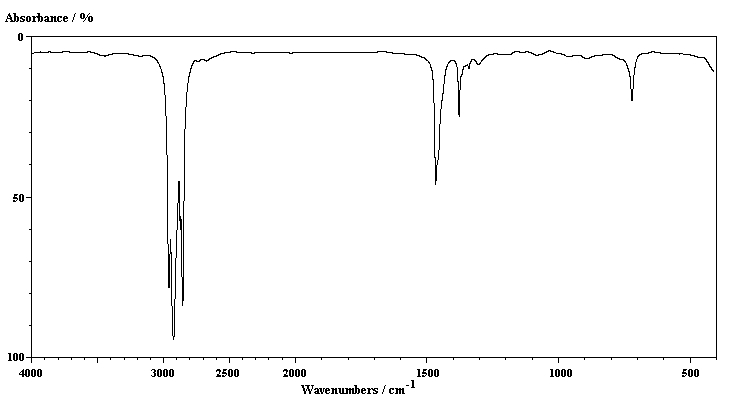
\includegraphics[width=0.49\linewidth]{Alkane} & 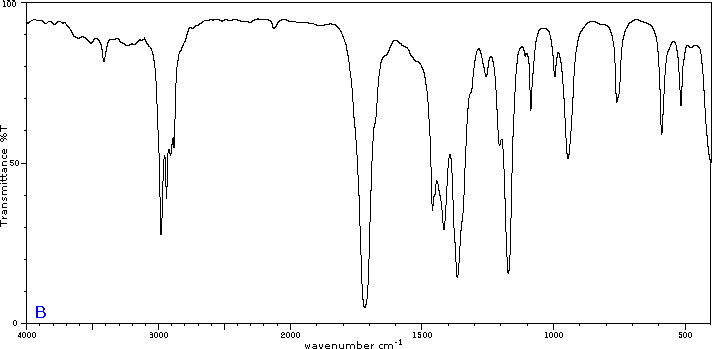
\includegraphics[width=0.49\linewidth]{Ketone} \\ \midrule
		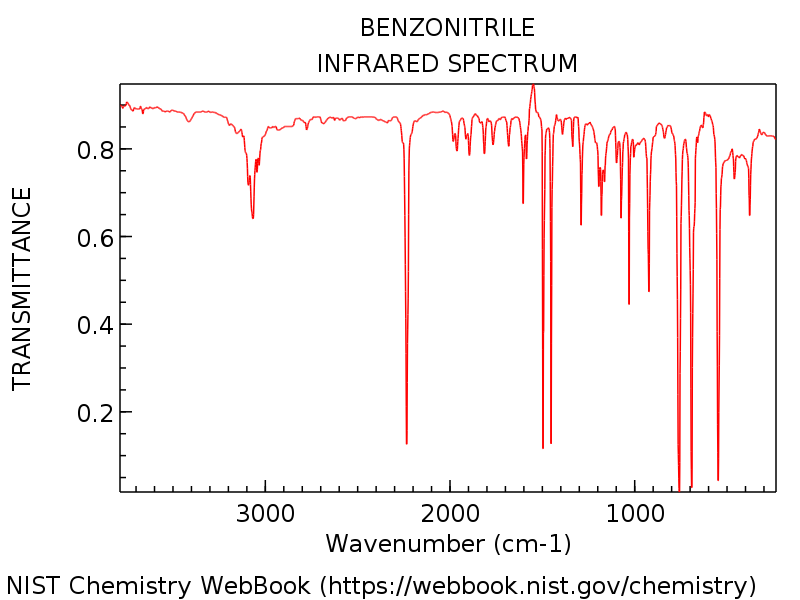
\includegraphics[width=0.49\linewidth, trim = 0 0 0 40, clip]{Nitrile} & 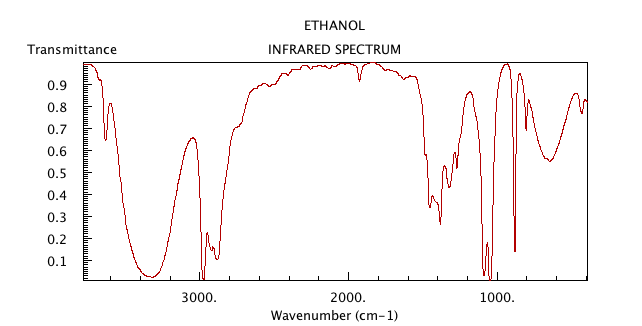
\includegraphics[width=0.49\linewidth, trim = 25 0 40 32, clip]{Alcohol}
	\end{tabular}
	
	\newpage
	\section*{Problem 2 (20 points)}
	Below is a microwave spectrum of the CN radical
	
	\noindent
	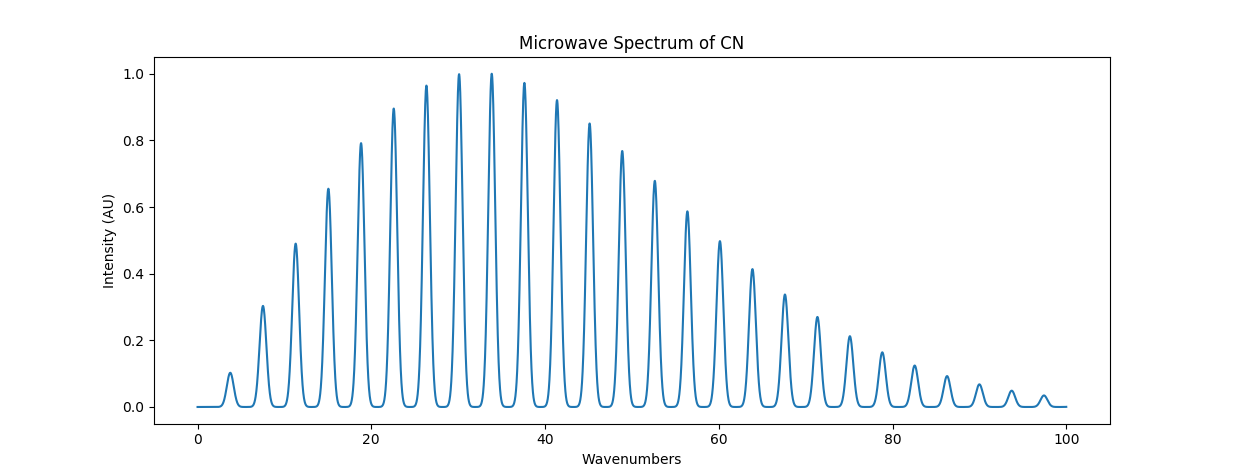
\includegraphics[trim= 40 0 40 0, clip=true, width=\linewidth]{CN_Microwave}
	
	\noindent
	Using the spectrum, find the following quantities:
	\begin{enumerate}
		\item $\tilde{B}$
		\item $r$ (Bond length)
		\item Temperature
	\end{enumerate}

	\newpage
	\section*{Problem 3 (10 points)}	
	Below IR and Raman spectra of the CN radical. Annotate them by labeling the following:
	\begin{enumerate}
		\item O, P, Q, R, and S branches
		\item Initial and final states for the first 3 transitions in each branch
		\item $\tilde{\nu} -2\chi_e\tilde{\nu}$
		\item Spacing between peaks (in terms of $\tilde{B}$)
	\end{enumerate}

	\noindent
	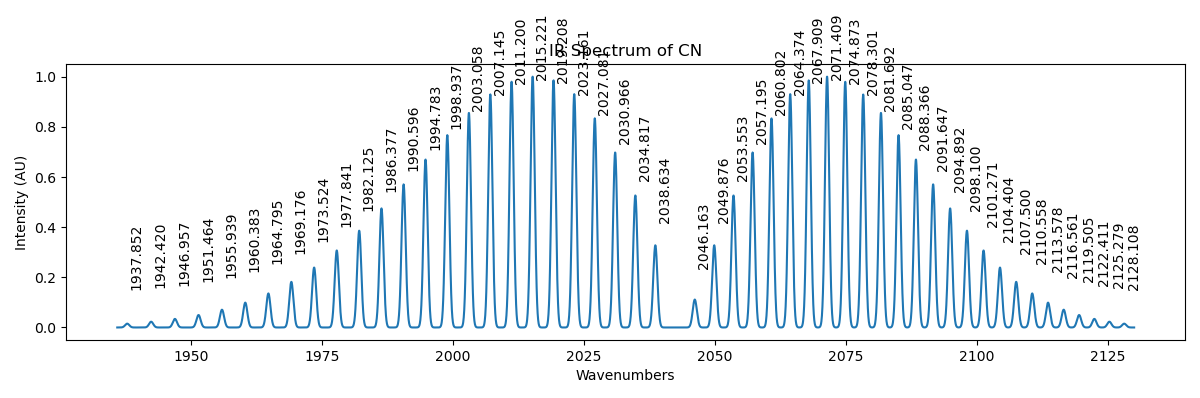
\includegraphics[trim= 60 0 60 0, clip=true, width=\linewidth]{CN_IR}
	
	\noindent
	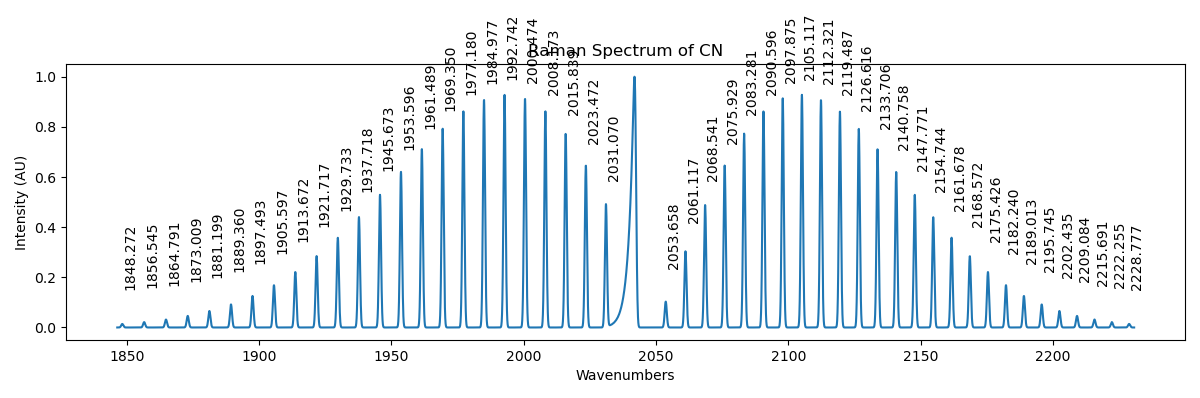
\includegraphics[trim= 60 0 60 0, clip=true, width=\linewidth]{CN_Raman}
	 
	\newpage
	\section*{Problem 4 (10 points)}
	Below is a table of the first few vibrational transitions for the CN radical
	
	\begin{tabular}{c|c}
		States & Energy ($cm^{-1}$) \\ \midrule
		$1\leftarrow0$ & $2042.416$ \\
		$2\leftarrow1$ & $2016.242$ \\
		$3\leftarrow2$ & $1990.068$ \\
		$4\leftarrow3$ & $1963.894$ \\
		$5\leftarrow4$ & $1937.720$ \\
	\end{tabular}

	\noindent
	Draw or print a Birge-Sponer plot and give the following quantities:
	\begin{enumerate}
		\item $\tilde{\nu}$
		\item $\chi_e$
		\item $\tilde{D}_e$
		\item $\tilde{D}_0$
	\end{enumerate}
	
\end{document}
	